%----------------------------------------------------------------------------------------
%	PAPER SETUP
%----------------------------------------------------------------------------------------

\newcommand*{\mytitle}{Beyond Passwords? Authentication with FIDO2 and WebAuthn} % Paper Title
\newcommand*{\myauthor}{Nils Siegle} % Paper Author
\newcommand*{\mydate}{May 2020} % Publication Date
\newcommand*{\myorg}{Applied Concepts of Web Engineering} % Organization, Journal, Subject this paper was published in


%----------------------------------------------------------------------------------------
%	PACKAGES AND OTHER DOCUMENT CONFIGURATIONS
%----------------------------------------------------------------------------------------

\documentclass[twoside,twocolumn]{article}

\usepackage{blindtext} % Package to generate dummy text throughout this template 

% ------- FONTS -------
\usepackage[sc]{mathpazo} % Use the Palatino font
\usepackage[T1]{fontenc} % Use 8-bit encoding that has 256 glyphs
\usepackage[utf8]{inputenc}

\linespread{1.05} % Line spacing - Palatino needs more space between lines
\usepackage{microtype} % Slightly tweak font spacing for aesthetics

\usepackage[english]{babel} % Language hyphenation and typographical rules

% ------- DOCUMENT MARGINS -------
\usepackage[hmarginratio=1:1,top=32mm,columnsep=20pt]{geometry} % Document margins
\usepackage[hang, small,labelfont=bf,up,textfont=it,up]{caption} % Custom captions under/above floats in tables or figures
\usepackage{booktabs} % Horizontal rules in tables
\usepackage{graphicx}

\usepackage{lettrine} % The lettrine is the first enlarged letter at the beginning of the text

% ------- LISTS -------
\usepackage{enumitem} % Customized lists
\setlist[itemize]{noitemsep} % Make itemize lists more compact

% ------- ABSTRACT -------
\usepackage{abstract} % Allows abstract customization
\renewcommand{\abstractnamefont}{\normalfont\bfseries} % Set the "Abstract" text to bold
\renewcommand{\abstracttextfont}{\normalfont\small\itshape} % Set the abstract itself to small italic text

% ------- SECTION TITLES -------
\usepackage{titlesec} % Allows customization of titles
\renewcommand\thesection{\Roman{section}} % Roman numerals for the sections
\renewcommand\thesubsection{\roman{subsection}} % roman numerals for subsections
\titleformat{\section}[block]{\large\scshape\centering}{\thesection.}{1em}{} % Change the look of the section titles
\titleformat{\subsection}[block]{\large}{\thesubsection.}{1em}{} % Change the look of the section titles

% ------- HEADERS AND FOOTERS -------
\usepackage{fancyhdr} % Headers and footers
\pagestyle{fancy} % All pages have headers and footers
\fancyhead{} % Blank out the default header
\fancyfoot{} % Blank out the default footer
\fancyhead[C]{\mytitle\, $\bullet$ \mydate\, $\bullet$ \myorg} % Custom header text
\fancyfoot[RO,LE]{\thepage} % Custom footer text

\usepackage{titling} % Customizing the title section

% ------- HYPERREF -------
\usepackage{hyperref} % For hyperlinks in the PDF
\AtBeginDocument{
  \hypersetup{pdftitle={\mytitle}} % Set the PDF's title to your title
  \hypersetup{pdfauthor={\myauthor}} % Set the PDF's author to your name
  \hypersetup{hidelinks} % Prints all links black; comment out for default LaTeX behavior
}

% ------- BIBTEX -------
\usepackage[backend=bibtex,style=numeric,citestyle=numeric,natbib=true]{biblatex}
\addbibresource{sources.bib}

\usepackage[autostyle=true]{csquotes}

% ------- COLORS -------
% Define colors for highlighting
\usepackage{xcolor}
\definecolor{lstbg}{gray}{0.95}
\definecolor{lstComment}{RGB}{51, 102, 0}
\definecolor{lstKey}{RGB}{0, 51, 204}
\definecolor{lstStr}{RGB}{162, 43, 43}

% ------- ACRONYMS -------
% \usepackage[nohyperlinks]{acronym} % Prints only used acronyms in overview
\usepackage[nohyperlinks, printonlyused]{acronym} % Prints only used acronyms in overview


%------------------------------------------------
%	CODE LISTINGS
%------------------------------------------------
\usepackage{listings}

% Load required languages
\lstloadlanguages{Python}

% Styling
\lstset{
  showtabs=false,
  showspaces=false,
  showstringspaces=false,
  basicstyle=\ttfamily,
  numbers=left, numberstyle=\tiny,
  columns=fullflexible,
  frame=single,
  breaklines=true,
  % prebreak={\\},
  backgroundcolor=\color{lstbg},
  commentstyle=\color{lstComment},
  stringstyle=\color{lstStr},
  keywordstyle=\color{lstKey},
  literate=
  {á}{{\'a}}1 {é}{{\'e}}1 {í}{{\'i}}1 {ó}{{\'o}}1 {ú}{{\'u}}1
  {Á}{{\'A}}1 {É}{{\'E}}1 {Í}{{\'I}}1 {Ó}{{\'O}}1 {Ú}{{\'U}}1
  {à}{{\`a}}1 {è}{{\`e}}1 {ì}{{\`i}}1 {ò}{{\`o}}1 {ù}{{\`u}}1
  {À}{{\`A}}1 {È}{{\'E}}1 {Ì}{{\`I}}1 {Ò}{{\`O}}1 {Ù}{{\`U}}1
  {ä}{{\"a}}1 {ë}{{\"e}}1 {ï}{{\"i}}1 {ö}{{\"o}}1 {ü}{{\"u}}1
  {Ä}{{\"A}}1 {Ë}{{\"E}}1 {Ï}{{\"I}}1 {Ö}{{\"O}}1 {Ü}{{\"U}}1
  {â}{{\^a}}1 {ê}{{\^e}}1 {î}{{\^i}}1 {ô}{{\^o}}1 {ß}{{\ss}}1
}

% Better highlighting for inline code
\newcommand{\linecode}[1]{%
  \colorbox{lstbg}{\textcolor{lstStr}{\textbf{\texttt{#1}}}}%
}

%----------------------------------------------------------------------------------------
%	TITLE SECTION
%----------------------------------------------------------------------------------------

\setlength{\droptitle}{-4\baselineskip} % Move the title up

\pretitle{\begin{center}\Huge\bfseries} % Article title formatting
\posttitle{\end{center}} % Article title closing formatting
\title{\mytitle} % Article title
\author{%
  \textsc{Nils Siegle} \\[1ex] % First author's name
  \normalsize 3087271 \\ % First author's institution
  \normalsize \href{mailto:nils.siegle@stud.uni-due.de}{nils.siegle@stud.uni-due.de} % First author's email address
}
\date{\today} % Leave empty to omit a date
\renewcommand{\maketitlehookd}{%

%------------------------------------------------
%	ABSTRACT
%------------------------------------------------

\begin{abstract}
\noindent \blindtext
\end{abstract}
}

%----------------------------------------------------------------------------------------

\begin{document}

% Print the title
\maketitle

\newpage
\onecolumn
%------------------------------------------------
%	ToC
%------------------------------------------------
\tableofcontents
\newpage

%------------------------------------------------
%	ACRONYMS
%------------------------------------------------

\section*{Abbreviations}
\begin{acronym}[AAAAAA]
  \acro{2fa}[2FA]{Two-Factor Authentication}
  \acro{authn}[authn]{Authentication}
  \acro{authz}[authz]{Authorization}
  \acro{api}[API]{Application Programming Interface}
  \acro{ctap}[CTAP]{Client to Authenticator Protocol}
  \acro{ctap2}[CTAP2]{Client to Authenticator Protocol2}
  \acro{fido}[FIDO]{Fast IDentity Online}
  \acro{fido2}[FIDO2]{Fast IDentity Online 2}
  \acro{hotp}[HOTP]{HMAC-based One-time Password}
  \acro{http}[HTTP]{Hypertext Transport Protocol}
  \acro{https}[HTTPS]{Hypertext Transport Protocol Secure}
  \acro{it}[IT]{Information Technology}
  \acro{mfa}[MFA]{Multi-Factor Authentication}
  \acro{nist}[NIST]{National Institute of Standards and Technology}
  \acro{nfc}[NFC]{Near-Field Communication}
  \acro{os}[OS]{Operating System}
  \acro{tpm}[TPM]{Trusted Platform Module}
  \acro{totp}[TOTP]{Time-based One-time Password}
  \acro{u2f}[U2F]{Universal Second Factor}
  \acro{uaf}[UAF]{Universal Authentication Framework}
  \acro{w3c}[W3C]{World Wide Web Consortium}
\end{acronym}

% \newacro{id}[ABRV]{Abbreviation}
% \acro{}[]{}
% Use 
% - \ac{id} for standard behavior
% - \acs{id} for acronym
% - \acl{id} for long version
% - \acp{id} for plural (with 's' at the end)

\newpage
\twocolumn

%----------------------------------------------------------------------------------------
%	ARTICLE CONTENTS
%----------------------------------------------------------------------------------------

% Section 1 - Introduction
\section{Introduction}
\label{sec:intro}

\lettrine[nindent=0em,lines=3]{T}his is an introduction with a fancy first letter. \blindtext

\begin{displayquote}
    \textbf{R:} \emph{What is our research question?}
\end{displayquote}

\blindtext


% Section 2 - Foundations
% ---------- SECTION II - METHODS ----------

\section{Methods}
\label{sec:methods}

To get detailed information about the current body of knowledge regarding \ac{fido2} and to answer the research question, a three-phased literature review is conducted.\\
The first phase is an unstructured internet search using common search engines like Google\footnote{https://google.com} or DuckDuckGo\footnote{https://duckduckgo.com/}. The aim of these searches is to get a basic understanding of what \ac{fido2} is, how it works, and how it is perceived in different media outlets.\\
These findings enable the second phase, a structured search for scientific literature regarding different subtopics or aspects of the FIDO-Framework, password-based authentication and other foundations. It makes use of more research-oriented search engines like Google Scholar\footnote{https://scholar.google.com/}, ScienceDirect\footnote{https://www.sciencedirect.com/}, IEEE Xplore\footnote{https://ieeexplore.ieee.org/}, AISeL\footnote{https://aisel.aisnet.org/} and the official FIDO Alliance whitepaper page\footnote{https://fidoalliance.org/white-papers/}.\\
In the last phase a search for secondary literature is conducted in the results of phase two, aiming for related scientific research on the topic.\\
\\
To answer the research question the framework proposed by Bonneau et al. (2012) \cite{bonneau2012} is used as a base, as the different benefits used for evaluating authentication methods are often referred in literature. However, the dimension \emph{Deployability} is dropped, leaving a focus on \emph{Usability} and \emph{Security} as proposed in the research question.\\
Those two parts are again supported by using other evaluation frameworks. For usability this will be the categorization proposed by Nielsen (1993) to make sure all aspects of acceptability and usability are covered. The security section is backed by a guide from the \ac{owasp}, more specifically the second vulnerability in the 2017 edition of \acp{owasp} Top 10, \emph{Broken Authentication}.

% Section 3 - Methods
% ---------- SECTION III - FOUNDATIONS ----------
% - [] Authentication and Authorisation
% - [] Password-based auth

\section{Foundations}
\label{sec:foundations}

The following chapter explains some basic concepts of web authentication, digital identities and the basic functionality of the \ac{fido2} framework.

% ---- Authn and Authz ----
\subsection{Authentication and Authorisation}
\label{subsec:authn_authz}

\ac{authn} and \ac{authz} are concepts present in virtually every protected \ac{it} ressource.
The former describes the process of identifying a user by verifying their digital identity, hence checking their \emph{authenticity}. Oftentimes only certain users are \emph{authorized} to access a protected ressource (e.g. specific parts of a website, sensitive data etc.). Therefore, an authorization has to take place both to ensure that the correct information is distributed to each user, and that no one without permission is able to manipulate data.\\
The most common and widespread type of web authentication is the so-called password-based authentication. In this case a user has to provide a \emph{username} (oftentimes an e-mail address, as these are globally unique) and a \emph{password} or \emph{passphrase}, a secret string only known to the user.\\
Only the correct combination of username and password grants access to the protected resource.\\
\\
In the above case the password is also referred to as an \emph{authentication factor}, of which there are three categories \cite{turner2016}:

\begin{description}
    \item[Knowledge factors] Something (only) the user knows like a password/-phrase or a \ac{pin}
    \item[Ownership factors] Something the user owns like a smart card or a \ac{totp} token
    \item[Inherence factors] Mostly biometric factors like fingerprints
\end{description}

This classification allows for a basic evaluation of possible \ac{authn} factors: While inherence factors are almost always available (the user carries them around), they often require special hardware like fingerprint sensors and are therefore not best suited for web authentication.\\
Ownership factors on the other hand are less resilient against (physical) theft - if the smartphone or hardware token is stolen, the attacker could authenticate.\\
The security of passwords and other knowledge factors is dependent on the users and how they store and generate them. Reusing passwords or using obvious, common or dictionary-based strings is undeniably less secure than using long, randomly generated ones stored in a password manager \cite{lyastani2018,hunt2011,hunt2018c}. Therefore, application developers have little influence on the security of possibly very important accounts, and if they try to enforce strong passwords by using arbitrary requirements, this can easily backfire \cite{hunt2017} and just decrease usability instead of increasing security. For that reason, the \ac{nist} has dropped all recommendations to use password complexity requirements and instead suggests to rely on length and black lists of known (and therefore insecure) passwords \cite{nist}.

% ---- MFA ----
\subsection{Multi-Factor Authentication}
\label{subsec:mfa}

% - Often \ac{2fa} using \ac{hotp} or \ac{totp}
% - Also possible with key files
% - Only guessing or stealing the password is not enough
To counter the security problems inherent to each single factor, \ac{mfa} can be used for further securing any authentication process by requiring more than one factor. Often this is realized as a \ac{2fa} using a normal password (knowledge factor) as the first, and some kind of \ac{otp} (for example \ac{totp}, \ac{hotp} or an SMS/eMail-Code) as the second.\\
In this case knowing the password of an account is not sufficient for logging in; a possible attacker would also have to get access to the device generating or receiving the second factor, often the users phone (ownership factor) \cite{statista_2fa,hunt2018a}.\\
It is important for \ac{mfa} in general that at least two of these factors are in different categories (e.g. a knowledge and an ownership factor) and at least one of them is not reusable (i.e. a \ac{otp}) \cite{nist,turner2016}.\\
\\
Using multiple factors can protect accounts against standard brute-force attacks like credential stuffing, where an attacker tries many combinations of known usernames and popular passwords.\\
However, \ac{mfa} is not a reliable protection against phishing attacks \cite{lyastani2020}, because a malicious site can easily fake an input field for \acp{otp}.


% ---- FIDO2 \& WebAuthn ----
\subsection{FIDO2 Overview}
\label{subsec:fido2_webauthn}

The \ac{fido} Alliance was founded in 2012 by a consortium of software and hardware companies with the goal to create an open, universal authentication framework. In December of 2014 the specifications for \acl{uaf}, a protocol for passwordless authentication, and \acl{u2f}, a protocol designed for second factors, were published by the alliance. The experiences from those protocols were later condensed into the \ac{fido2} framework, launched only recently in April of 2018 \cite{fido_history}.\\
\\
\ac{fido2} aims to provide a strong authentication factor (either as single factor for passwordless login or in a \ac{mfa} setting) using hardware keys, so called \emph{authenticators}. Those can be on the device itself (for example using \emph{Windows Hello}, Apples \emph{TouchID} or a \ac{tpm} chip), and therefore \emph{internal} authenticators. The alternative are external or \emph{roaming} authenticators, often realised as USB keys or \ac{nfc} cards.\\
The party providing the protected ressource (e.g. a website or other web application) is referred to as \emph{relying party}.\\
The \ac{fido2} Framework consists mainly of two components: The \emph{WebAuthn} web \ac{api}, standardized by the \ac{w3c}, is the interface between the browser or \ac{os} and the authentication servers of the relying party \cite{webauthn_standard}. WebAuthn is currently supported by the Windows 10 and Android \acp{os} as well as by the Google Chrome, Mozilla Firefox, Microsoft Edge and Apple Safari web browsers \cite{fido2_webauthn}.\\
The second part is the \ac{ctap2} protocol that is responsible for connecting roaming authenticators to the clients device (e.g. a smartphone, laptop or personal computer) \cite{fido2_overview,fido2_ctap}.\\

\begin{figure*}[!ht]
    \centering
    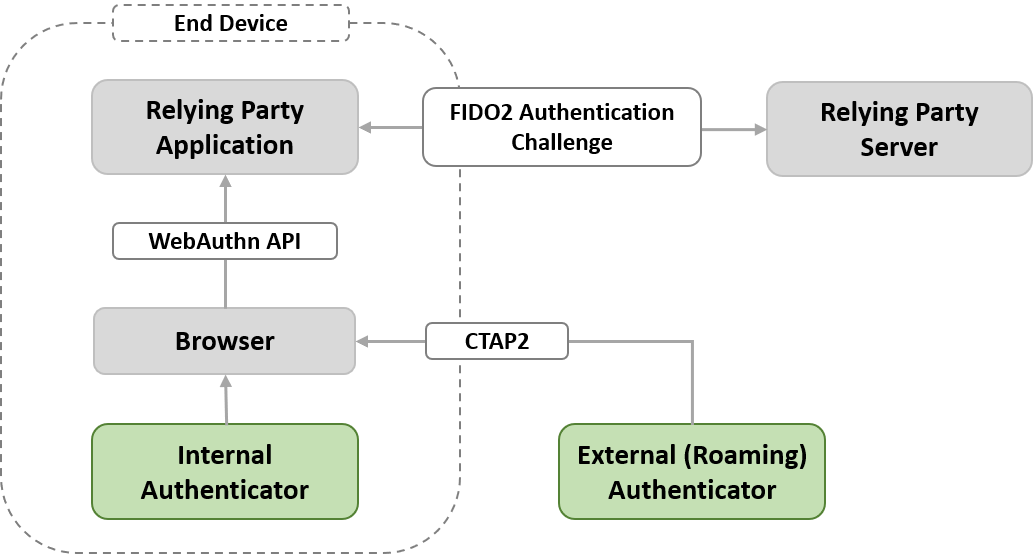
\includegraphics[width=1.8\columnwidth]{Figures/fido2_webauth_ctap_flow.png}
    \caption[FIDO2 Authentication Flow]{FIDO2 WebAuthn \& CTAP2 Authentication Flow}
    \label{fig:fido2_webauth_ctap_flow}
\end{figure*}

\noindent As seen in figure \ref{fig:fido2_webauth_ctap_flow}, the \ac{rp} will never know what kind of authenticator was used - as long as it can communicate over WebAuthn (or indirectly over \ac{ctap}).\\
The WebAuthn \ac{api} is used for two major operations: Either to register a new authenticator with an application, creating new public key credentials, or to login to one of these applications. For logging in, the \ac{rp} sends an \emph{authentication assertion}. The authenticator has to verify the presence and consent of the user, usually using a button or fingerprint sensor on the security key, before the assertion is signed with the correct private key and send back to the \ac{rp} \cite{webauthn_standard,mdn_webauthn}.

% Section 4 - Results
% ---------- SECTION IV - FIDO2 & WebAuthn ----------

\section{Results}
\label{sec:results}

To answer the research question, the literature is analyzed for two main topics: usability and security.\\
While there is some amount of research regarding the usability of \ac{fido2}, literature regarding the preceding protocols \ac{u2f} and \ac{uaf} is also taken into account due to the similarity of the involved hardware and authentication flows.\\
The security part of this chapter is mainly based on evaluations of the proposed concepts and mechanisms, as there is not yet any research regarding the security of actual implementations of either hardware or protocols.

% ---- Subsection Usability ----
\subsection{Usability}
\label{subsec:usability}

To determine whether a new authentication concept is accepted by users, and could therefore replace passwords, the usability plays a significant role. Regular passwords have been the prevalent authentication mechanism since the 1960's \cite{mcmillan2012}, so users are very familiar with their usage. The concept of sending credentials, checking them, and granting access to the protected ressource is also very intuitive. Using a hardware token, or in case of internal authenticators only a system dialogue, is a radically different approach.\\
A good starting point to evaluate whether this hardware-dependent approach is suitable is the study conducted by Lang et al \cite{lang2017}. The authors analyzed the roll-out of hardware tokens for 50,000 employees of Google as a second factor. In comparison to other \ac{2fa} methods like \ac{totp}, they found using a security key to be significantly faster.\\
On the other hand, a more qualitative and in-depth study of Das et al (2018) showed major usability problems for participants without technical backgrounds, especially during the initial setup. They report that users had trouble finding the correct instructions and where not able to intuitively use the device, as they had not yet developed a mental model regarding the functionality of the keys. The authors also explicitly state that one of the major problems was that users still had to enter their passwords, leading to additional work and complexity without any perceived benefit \cite{das2018}. This factor becomes less of a problem when a \ac{fido2} token is used for passwordless authentication.\\
\\
The most important scientific work for this section is a recent study by Lyastani et al, published in 2020, that focuses on the usability of \ac{fido2} as a means of passwordless, \ac{1fa}. They conclude that participants rated logging in via \ac{fido2} and an external authenticator as more usable than standard passwords, and were able to show a higher acceptance than the latter \cite{lyastani2020}.\\
However, the authors also identified some challenges, of which the most important ones are listed below:

\begin{description}
    \item[Complex Setup] Especially the initial registration of the key was seen as a challenge by many participants, this corresponds with the findings of \cite{das2018}.
    \item[Requires Physical Device] Users criticized that they had to carry an authenticator, and that the absence of this devices effectively logs them out of the application, substantially limiting spontaneous use.
    \item[Support of Other Devices] Logging in on devices without any way to connect the authenticator (e.g. a tablet or public PC without USB-A ports or NFC) is impossible.
    \item[Account Recovery after Loss] If the security key gets lost or stolen, account recovery is much more complex than with passwords. The current recommendation is to register a second backup key with each account \cite{gomi2019}.
    \item[No Account Delegation] It is not possible to grant a trusted third party (e.g. a colleague) access to an account without giving away the hardware key.
\end{description}

% \noindent Nonetheless, Lyastani et al could also 

% - Google Advanced Protection\footnote{https://landing.google.com/advancedprotection/})

% ---- Subsection Security ----
\subsection{Security}
\label{subsec:security}

From a security point of view we can mainly analyze the concepts behind the protocols in the \ac{fido2} framework, as there is not yet any research regarding actual protocol implementations or hardware. Therefore, this section is mainly based on the official documentation and first evaluations of security researches. Additionally, we will look mostly at using \ac{fido2} in the passwordless, single factor mode.\\
The main difference to standard passwords is the use of public-key cryptography instead of storing a shared secret. For every new application the authenticator generates a separate key pair, of which only the public key is stored within the \acp{rp} servers. This has two implications: First, different credentials are used for every service, which means accounts cannot be linked across services based on the key, and as the user has no influence on the key generation, there is no way to derive user information from the public key. Second, as no secret is stored on the RPs side, a credential leak has no effect - knowing the public key is of no use for taking over an account. In addition to that resilience against credential leaks, the public-key infrastructure also prevents against phishing. Even if, for example, a malicious website could forge a \ac{fido2} authentication challenge using stolen public keys, the challenge response can not be used to login to the real account.\\
In general, public-key infrastructures are considered very robust and mature, although their security depends on the algorithm and key length used.\\
\\
While the protocols and general authentication flow can be seen as very secure and less prone to various attacks than passwords, another big factor of the general security are the authenticators themselfs. In all cases, it should not be possible to extract the private keys from the authenticator. Additionally, the presence and consent of the user has to be determined for every login, meaning the person has to physically act by pressing a button or accepting a system dialog. This ensures that malicious services cannot trigger and sign assertions without the users knowledge. Many authenticators, like the popular YubiKey 5, also implement another factor like a \ac{pin} or a fingerprint sensor to further protect against theft \cite{yubikey_5_nfc}.
% - Public-Key-Cryptography
% - No Phishing, Replay or data breaches possible
% - Keys are Read-Only
% - Require physical presence or even PIN/Biometrics
% - NO resilience to theft
% -> Hardware key can be secured using PIN/Fingerprint, adding knowledge/inheritance factor


% ---- Subsection Other ----
\subsection{Comparison}
\label{subsec:comparison}

The below comparison of passwords, FIDO2 passwordless login and FIDO U2F is based on the authentication method evaluation framework developed by Bonneau et al \cite{bonneau2012}. The evaluation of simple passwords, also proposed by the former authors and supported by others \cite{lyastani2020} is not changed.

\begin{figure*}[ht]
    \centering
    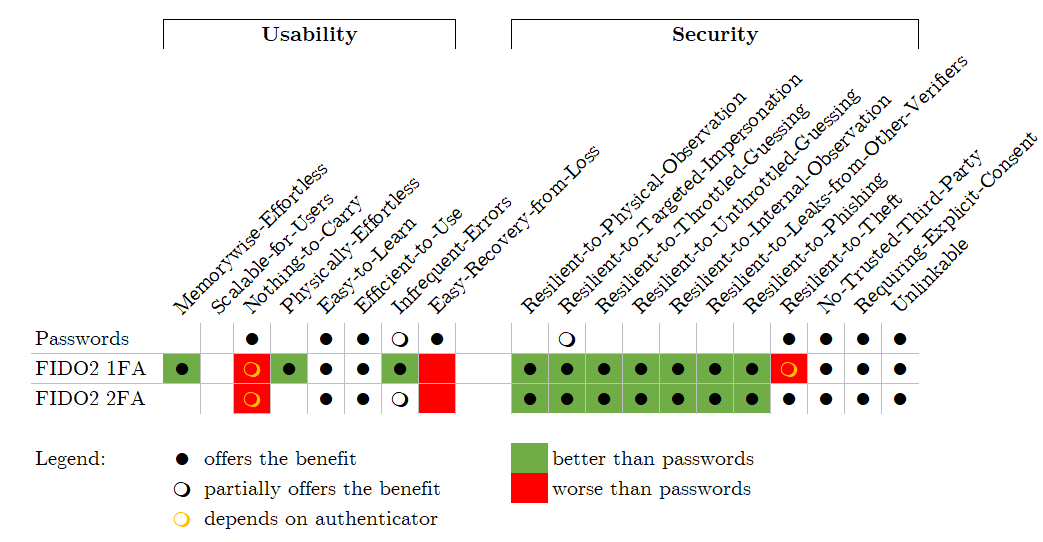
\includegraphics[width=1.8\columnwidth]{Figures/bonneau_matrix.png}
    \caption[Comparison of Authentication Methods]{Comparison of standard passwords with FIDO 1FA/2FA using a modified version of the framework proposed by Bonneau et al (2012)}
    \label{fig:bonneau_matrix}
\end{figure*}

\noindent As figure \ref{fig:bonneau_matrix} shows, both \ac{fido2} modes score exceptionally well. In fact, as is also mentioned in \cite{lyastani2020}, no other authentication method offers as many benefits as the former.

% Section 5 - Discussion
% ---------- SECTION V - Discussion ----------

\section{Discussion}
\label{sec:discussion}

% ---- Subsection Threats to Validity ----
\subsection{Threats to Validity}
\label{subsec:validity_threats}

% Section 6 - Conclusion
% ---------- SECTION VI - CONCLUSION ----------

\section{Conclusion}
\label{sec:conclusion}

\ac{fido2} shows some very good potential to solve many of todays most pressing problems regarding password-based authentication. It is a open framework, based on an open specification by the \ac{w3c}, supported by browser and operating system vendors as well as many application providers. This broad support could, step by step, introduce many people to new concepts of authentication.\\
But the biggest factor in whether or not \ac{fido2} will actually become successful will remain user acceptance. For now, most of these users have not yet been directly affected by credential leaks, which lowers the perceived necessity for any changes, especially such breaking ones.\\
Or, as security researcher Troy Hunt put it in an article called "Here's Why [Insert Thing Here] Is Not a Password Killer" \cite{hunt2018a}:

\begin{displayquote}
    \emph{Every single solution I've seen that claims to "solve the password problem" just adds another challenge in its place thus introducing a new set of problems.}
\end{displayquote}

\noindent For the start, \ac{fido2} might be a good method for secure authentication in business environments. In such a case, the amount of accounts secured is rather low, while the potential business impact in case of stolen accounts can be exceptionally high. The local IT could coordinate the roll-out and provide support, thus increasing acceptability, as shown by \cite{lang2017}.\\
\\
Future research should focus on the long-term usability of the framework, to show if and how fast users get accustomed to the new authentication concepts, how often account recovery actually becomes a problem, and what other challenges may arise in day-to-day use. Additionally, further research is needed regarding the security of both the protocol implementations and roaming as well as internal authenticators.\\
\\
For security-conscious persons willing to invest some money and time for setting up a fast, secure and easy-to-use authentication method, \ac{fido2} could be a very good alternative to other single- and multi-factor authentication methods.

% Single column layout for the rest of the paper
\onecolumn

%----------------------------------------------------------------------------------------
%  BIBLIOGRAPHY
%----------------------------------------------------------------------------------------
\printbibliography[heading=bibintoc]

%------------------------------------------------

% Section 5 - Appendix
% ---------- SECTION VII - APPENDIX ----------

\section{Appendix}
\label{sec:appendix}

% ---- Appendix I ----
\subsection{Appendix I}
\label{apx_1}


%----------------------------------------------------------------------------------------

\end{document}
